\begin{frame}[fragile]{Milestoning: Temporal Coarse-Graining of MD}
\begin{tikzpicture}[scaleall=1.0]
\pcuad{\textwidth}{\textheight}
%\showcuad
\path(nw) +(-0.75,0.15) node(text)[anchor=north west,text 
width=\textwidth]{{\tiny \textcolor{red!80!black}{A. K. Faradjian and R. Elber {\it J Chem Phys} {\bf 120}:010880 (2004).}}};
\path(nw) +(-0.75,-0.5) node(text1)[anchor=north west,text width=0.5\textwidth]{
Coarsening of a hypothetical infinitely long MD trajectory onto a \textcolor{red}{jump process}};
\path(nw) +(-0.75,-2) node(image1)[anchor=north west]{
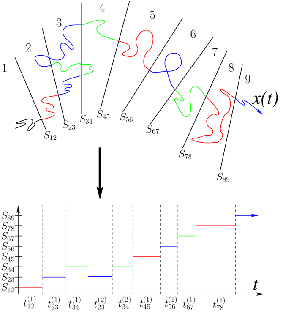
\includegraphics[width=0.5\textwidth]{milestoning1}};
\path(nw) +(5,0) node(text2) [anchor=north west,text width=0.5\textwidth]{
\begin{center}
Coarse-grained kinetics are fully described by a \textcolor{blue}{rate matrix}:
\end{center}
\begin{displaymath}
q_{ik,ij} = \left\{\begin{array}{ll}
\frac{\ds N_{ik,ij}}{\ds R_{ij}} & \mbox{if}\ R_{ij}>0;\\
0 & \mbox{if}\ R_{ij}=0,
\end{array}\right.
\end{displaymath}
where
\begin{align*}
N_{ik,ij} =& \left\{\begin{array}{l}
\mbox{\# of times trajectory}\\
\mbox{collides with $S_{ik}$ after}\\
\mbox{last hitting $S_{ij}$}
\end{array}\right\},\\
R_{ij} = &\left\{\begin{array}{l}
\mbox{total amount of time for}\\
\mbox{which $S_{ij}$ was the last}\\
\mbox{milestone hit}
\end{array}\right\},\\
& = \sum_m t_{ij}^{(m)}.
\end{align*}
};
\end{tikzpicture}
\end{frame}

